% Implementation report adapted from the IEEEtran bare_conf.tex structure
% supplied by Luis F. Recalde. Original template: Michael Shell, V1.4b (2015).
% This renamed manuscript contains new text, equations, figures, and experiments.
\documentclass[conference]{IEEEtran}
\usepackage[T1]{fontenc}
\usepackage{amsmath,amssymb,bm}
\usepackage{graphicx,booktabs,array}
\usepackage{xcolor}
\usepackage{balance}
\definecolor{lightpink}{RGB}{0,90,200}
\usepackage[colorlinks=true,linkcolor=lightpink,citecolor=lightpink,urlcolor=lightpink]{hyperref}
\hypersetup{
 pdftitle={Constrained Control Allocation for Dynamic Ship Positioning Using an Encoder-Decoder Neural Network},
 pdfauthor={Luis F. Recalde},
 pdfkeywords={control allocation, ship dynamics, nonlinear programming, recurrent neural network}
}
\graphicspath{{figures/}}
\DeclareGraphicsExtensions{.pdf}
\newcommand{\RR}{\mathbb{R}}
\DeclareMathOperator*{\argmin}{arg\,min}
\DeclareMathOperator{\diag}{diag}
\newcommand{\pos}[1]{\left[#1\right]_{+}}
\newcommand{\norm}[1]{\left\lVert#1\right\rVert}
\newcommand{\T}{^{\mathsf T}}
\newcommand{\ud}{\bm{u}}
\newcommand{\taud}{\bm{\tau}^{d}}
\newcommand{\tauc}{\bm{\tau}^{\mathrm{cmd}}}
\newcommand{\tauh}{\hat{\bm{\tau}}}
\newcommand{\uh}{\hat{\bm{u}}}
% Expand generated rows without LaTeX's file hooks starting an empty table row.
\makeatletter
\let\inputtable\@@input
\makeatother
% Generated by write_tables.py; do not edit numerical values here.
\newcommand{\NNMedian}{0.308}
\newcommand{\NLPMedian}{7.955}
\newcommand{\EncoderParameters}{51,269}
\newcommand{\TotalParameters}{102,920}
\newcommand{\SelectedEpoch}{41}
\newcommand{\ForbiddenSamples}{214,119}
\newcommand{\ForbiddenPercent}{21.41}
\newcommand{\CPUModel}{Intel Core i9-14900HX}
\newcommand{\TorchVersion}{2.5.1+cpu}
\newcommand{\CasadiVersion}{3.7.2}
\newcommand{\TimingRatio}{25.8}
\newcommand{\NLPFailures}{0}

\hyphenation{op-ti-mi-za-tion allo-ca-tion re-con-struc-tion}

\begin{document}
\raggedbottom
\title{Constrained Control Allocation for Dynamic Ship Positioning Using an Encoder--Decoder Neural Network}
\author{
  \IEEEauthorblockN{Luis F. Recalde}
  \IEEEauthorblockA{School of Robotics Engineering\\
  Worcester Polytechnic Institute\\
  Worcester, Massachusetts, USA}
}
\maketitle

\begin{abstract}
This work presents the implementation and evaluation of a recurrent neural
network for constrained control allocation of a ship with one tunnel thruster
and two azimuth thrusters. Following the encoder--decoder formulation of
Skulstad et al., the encoder outputs three thrust forces and two azimuth angles.
The training objective combines physical and learned force reconstruction
with actuator penalties. We generate one million smooth command samples
within prescribed magnitude and rate bounds. A nonlinear allocation problem
implemented in CasADi and solved with IPOPT provides the optimization baseline.
We evaluate force reconstruction, actuator violations, and allocation time.
On a 1,024-sample evaluation segment, the median allocation times are
\NNMedian~ms for the neural allocator and \NLPMedian~ms for the nonlinear
program. The results show that fast, accurate force reconstruction can still
be accompanied by actuator rate violations.
\end{abstract}
\IEEEpeerreviewmaketitle

\section{Introduction}
Dynamic positioning requires a vessel to generate the planar forces and yaw
moment requested by a motion controller. These generalized forces must be
distributed among the available thrusters while respecting their operating
limits. For a vessel with azimuth thrusters, the allocation variables include
both thrust magnitudes and orientations. The resulting mapping is nonlinear,
and several actuator configurations can produce the same generalized force.
Control allocation can therefore be formulated as an optimization problem
with actuator constraints and performance requirements.

Optimization-based methods provide a direct way to include actuator
saturation, rate limits, and power-related objectives.
Sequential quadratic programming is one established approach to nonlinear
allocation~\cite{Johansen2004}. In this report, the baseline is a nonlinear
program (NLP) formulated with CasADi~\cite{Andersson2019} and solved using
the interior-point method implemented in IPOPT~\cite{Wachter2006}.

An alternative is to learn the allocation map offline and evaluate a neural
network during operation. We take inspiration from
Skulstad et al.~\cite{Skulstad2023}, who use an autoencoder-like recurrent
network with force and actuator loss functions. The encoder outputs thruster
commands, which are mapped to generalized forces through a known allocation
model. This physical mapping gives the intermediate variables their
meaning as actuator commands.

The objective of this report is to implement and evaluate this recurrent
encoder--decoder allocator. Both allocation methods use the same signed
thruster offsets, actuator ordering, and force convention. All comparisons
use prescribed force requests in open loop, without a motion controller.

\section{Methodology}
\subsection{Notation and coordinate conventions}
Let $\mathcal F_n$ denote the inertial North--East frame and
$\mathcal F_b$ the ship-fixed frame, with $x_b$ forward, $y_b$ to starboard,
and $z_b$ downward. The planar pose and body velocity are
\begin{equation}
 \bm{\eta}=\begin{bmatrix}x_n&y_n&\psi\end{bmatrix}\T,\qquad
 \bm{\nu}=\begin{bmatrix}u&v&r\end{bmatrix}\T .
\end{equation}
We define the generalized-force vector in sway--surge--yaw order as
\begin{equation}
 \bm{\tau}=\begin{bmatrix}
 \tau_{\mathrm{sway}}&\tau_{\mathrm{surge}}&\tau_{\mathrm{yaw}}
 \end{bmatrix}\T .
 \label{eq:tauorder}
\end{equation}
Forces are expressed in N, yaw moments in N\,m, and angles in rad unless
stated otherwise.

\subsection{Ship dynamics}
We use the standard planar marine-craft model~\cite{FossenModel},
\begin{align}
 \dot{\bm{\eta}} &= \bm{R}(\psi)\bm{\nu},\\
 \bm{M}\dot{\bm{\nu}}+\bm{C}(\bm{\nu})\bm{\nu}
       +\bm{D}\bm{\nu} &= \bm{P}\bm{\tau},
 \label{eq:ship}
\end{align}
where $\bm M$, $\bm C$, and $\bm D$ are the inertia, Coriolis, and damping
matrices, respectively, and
\begin{equation}
 \bm{R}(\psi)=
 \begin{bmatrix}
 \cos\psi&-\sin\psi&0\\
 \sin\psi& \cos\psi&0\\
 0&0&1
 \end{bmatrix},\quad
 \bm{P}=\begin{bmatrix}0&1&0\\1&0&0\\0&0&1\end{bmatrix}.
\end{equation}
The permutation matrix $\bm P$ converts \eqref{eq:tauorder} to the
surge--sway--yaw order used in the dynamic equations.

The effective inertia and damping matrices have the structure
\begin{equation}
 \bm M=\begin{bmatrix}m_{11}&0&0\\0&m_{22}&m_{23}\\0&m_{23}&m_{33}\end{bmatrix},
 \qquad \bm D=\diag(d_{11},d_{22},d_{33}).
\end{equation}
Table~\ref{tab:ship} lists the coefficients adapted from the Gunnerus model
in the \href{https://github.com/rgmaidana/dysas/blob/master/DYSAS/Vessel.py}{Dynamic Systems Accident Simulator}.
The damping coefficients are positive under the sign convention in
\eqref{eq:ship}.

\begin{table}[t]
\caption{Effective ship-model parameters, rounded for presentation.}
\label{tab:ship}
\centering
\begin{tabular}{lll}
\toprule
Parameter&Value&Unit\\
\midrule
$m_{11}$&$3.48061\times10^5$&kg\\
$m_{22}$&$7.8061\times10^4$&kg\\
$m_{23}$&$-2.30000\times10^5$&kg\,m\\
$m_{33}$&$1.58304498\times10^6$&kg\,m$^2$\\
$d_{11}$&$1.7400\times10^4$&N\,s/m\\
$d_{22}$&$8.0200\times10^4$&N\,s/m\\
$d_{33}$&$4.9715\times10^6$&N\,m\,s/rad\\
\bottomrule
\end{tabular}
\end{table}

We define the state vector as $\bm x=[\bm\eta\T,\bm\nu\T]\T$ and integrate
\eqref{eq:ship} using fourth-order Runge--Kutta with a sampling time of
$\Delta t=0.05$~s.

\subsection{Allocation model}
The vessel has one tunnel thruster $T_1$ and two azimuth thrusters $T_2,T_3$.
The actuator command and thrust vectors are
\begin{equation}
 \ud=\begin{bmatrix}F_1&F_2&\alpha_2&F_3&\alpha_3\end{bmatrix}\T,
 \quad \bm F=\begin{bmatrix}F_1&F_2&F_3\end{bmatrix}\T.
 \label{eq:commands}
\end{equation}
Bold $\ud$ denotes actuator commands, while the scalar $u$ denotes surge
velocity. The signed thruster locations relative to the body origin are
\begin{equation}
 \bm r_1=\begin{bmatrix}l_2\\0\end{bmatrix},\quad
 \bm r_2=\begin{bmatrix}l_1\\l_3\end{bmatrix},\quad
 \bm r_3=\begin{bmatrix}l_1\\l_4\end{bmatrix},
\end{equation}
with
\begin{equation}
 l_1=-14,\qquad l_2=14.5,\qquad l_3=-2.7,\qquad l_4=2.7
 \quad [\mathrm m].
\end{equation}
These offsets follow~\cite{Skulstad2023}. The thruster configuration is
shown in Fig.~\ref{fig:geometry}.

\begin{figure}[t]
\centering
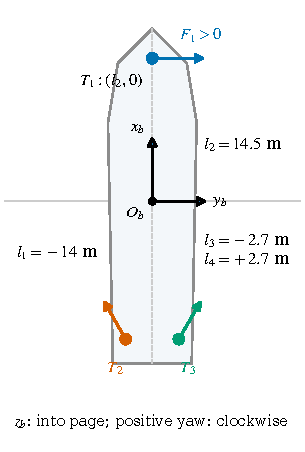
\includegraphics[height=2.9in]{ship_geometry}
\caption{Thruster locations and force directions in the ship-fixed frame.}
\label{fig:geometry}
\end{figure}

The mapping from actuator commands to generalized forces is
\begin{equation}
 \bm\tau=\bm g(\ud)=\bm B(\bm\alpha)\bm F,\qquad
 \bm\alpha=\begin{bmatrix}\alpha_2&\alpha_3\end{bmatrix}\T,
 \label{eq:allocation}
\end{equation}
where the allocation matrix is
\begin{equation}
 \bm B(\bm\alpha)=
 \begin{bmatrix}
 1&\sin\alpha_2&\sin\alpha_3\\
 0&\cos\alpha_2&\cos\alpha_3\\
 l_2&l_1\sin\alpha_2-l_3\cos\alpha_2&
      l_1\sin\alpha_3-l_4\cos\alpha_3
 \end{bmatrix}.
 \label{eq:B}
\end{equation}

\subsection{Actuator constraints}
Table~\ref{tab:bounds} summarizes the sampling ranges and the physical
magnitude and rate limits used for allocation. Each azimuth angle also
excludes the open sectors $(-100^\circ,-80^\circ)$ and
$(80^\circ,100^\circ)$; their endpoints are admissible.

\begin{table}[t]
\caption{Data-generation ranges and physical actuator limits.}
\label{tab:bounds}
\centering
\setlength{\tabcolsep}{4pt}
\begin{tabular}{lccc}
\toprule
Variable&Data range&Actuator range&Rate limit\\
\midrule
$F_1$ (N)&$\pm10000$&$\pm30000$&1000 N/s\\
$F_2,F_3$ (N)&$\pm5000$&$[-30000,60000]$&1000 N/s\\
$\alpha_2,\alpha_3$&$\pm180^\circ$&$\pm180^\circ$&$10^\circ$/s\\
\bottomrule
\end{tabular}
\end{table}

\subsection{Nonlinear allocation}
The control allocation problem is formulated as an NLP. Let
\begin{equation}
 \bm e_k=\bm B(\bm\alpha_k)\bm F_k-\taud_k
\end{equation}
denote the generalized-force allocation error. The cost $J_k(\ud_k)$
penalizes this error, thrust demand, and changes in azimuth angles, subject
to the actuator constraints. CasADi constructs the symbolic problem and
provides its derivatives. IPOPT solves the resulting nonconvex NLP,
initialized at each time step with the previous applied command.

\subsection{Constrained random-data generation}
We generate $N=10^6$ samples of \eqref{eq:commands} within the data ranges
in Table~\ref{tab:bounds}. Each channel uses an independent random stream.
Successive targets are connected by smooth quintic transitions whose
durations respect the rate limits. The angles cover the full sampling
range, including the forbidden sectors.

The generalized-force targets are computed using the allocation model:
\begin{equation}
 \taud_k=\bm g(\ud_k^{\mathrm{data}}),\qquad k=0,\ldots,N-1.
 \label{eq:datatau}
\end{equation}
We split the record chronologically into 800,000 training samples,
100,000 validation samples, and 100,000 evaluation samples.
Figure~\ref{fig:commandsdata} shows the generated commands.

\begin{figure*}[t]
\centering
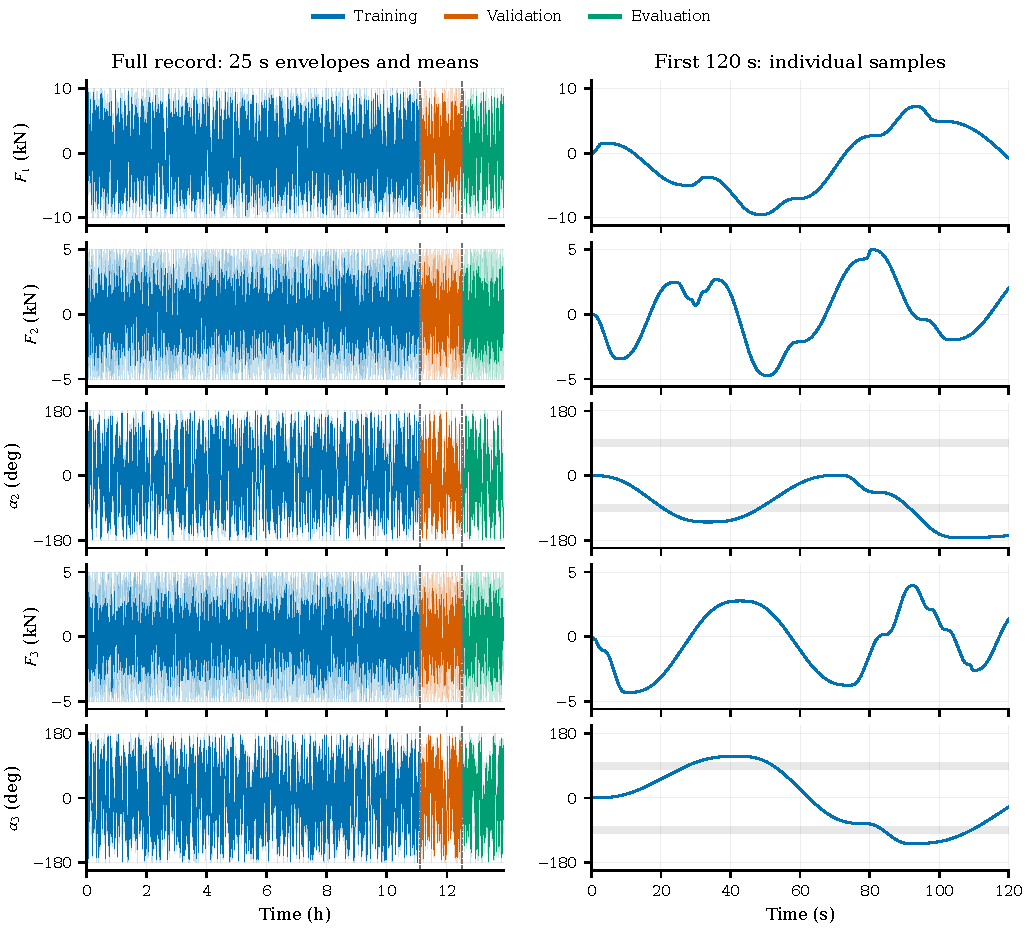
\includegraphics[width=.98\textwidth]{generated_commands}
\caption{One million generated command samples. Left: full-record envelopes
and block means. Right: the first 120~s, showing smooth transitions.
Shaded angular bands indicate forbidden sectors.}
\label{fig:commandsdata}
\end{figure*}

\section{Encoder--Decoder Deep Neural Network}
\subsection{Network structure and physical intermediate variables}
The network follows the recurrent encoder--decoder structure
in~\cite{Skulstad2023}. It maps the three-dimensional desired force
$\taud_k$ to five physical actuator commands $\uh_k$, from which the decoder
reconstructs a three-dimensional force $\tauh_k$. Each half contains two
64-unit LSTM layers and a linear output layer, as shown in
Fig.~\ref{fig:network}. The encoder's linear outputs are scaled by
$\bm S_u=\diag(10000,5000,\pi,5000,\pi)$ to obtain commands in N and rad.
The physical force is computed separately as $\tauc_k=\bm g(\uh_k)$.

\begin{figure*}[t]
\centering
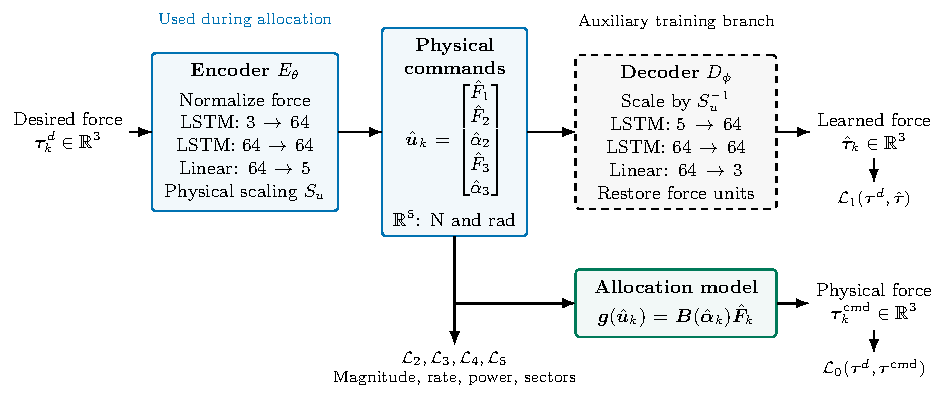
\includegraphics[width=.98\textwidth]{network_diagram}
\caption{Recurrent encoder--decoder with learned and physical force
reconstruction branches. The encoder outputs physical thruster commands.}
\label{fig:network}
\end{figure*}

\subsection{Cost function design}
Consider a batch containing $B$ ordered sequences of $T$ samples, with
$n=BT$. Let $\bm D_\tau=\diag(\bm\sigma_\tau)$, where $\bm\sigma_\tau$
contains the force standard deviations computed from the training data.

\subsubsection{Physical force reconstruction}
The encoder must produce commands whose physical force matches the request:
\begin{equation}
 \mathcal L_0=\frac{1}{3n}
 \sum_{b=1}^{B}\sum_{k=1}^{T}
 \norm{\bm D_\tau^{-1}
       \left(\tauc_{b,k}-\taud_{b,k}\right)}_2^2.
 \label{eq:L0}
\end{equation}
This term gives the intermediate variables their physical meaning,
following~\cite{Skulstad2023}. Accurate reconstruction by the learned
decoder alone would not ensure that the commands generate the requested force.

\subsubsection{Learned force reconstruction}
The decoder contributes
\begin{equation}
 \mathcal L_1=\frac{1}{3n}
 \sum_{b=1}^{B}\sum_{k=1}^{T}
 \norm{\bm D_\tau^{-1}
       \left(\tauh_{b,k}-\taud_{b,k}\right)}_2^2.
 \label{eq:L1}
\end{equation}
Both force errors use the same training standard deviations.

\subsubsection{Command magnitudes}
Define $[x]_+=\max(x,0)$. The symmetric training limits are
\begin{equation}
 \bm b_u=\begin{bmatrix}30000&60000&\pi&60000&\pi\end{bmatrix}\T
 \quad\text{in N and rad}.
\end{equation}
These follow the neural penalty in the reference formulation and differ
from the asymmetric stern-thrust limits in Table~\ref{tab:bounds}.
Using unit references $q_j=1$~N for forces and $q_j=1$~rad for angles,
\begin{equation}
 \mathcal L_2=\frac{1}{n}\sum_{b,k}\sum_{j=1}^{5}
 \frac{\pos{|\hat u_{b,k,j}|-b_{u,j}}}{q_j}.
 \label{eq:L2}
\end{equation}

\subsubsection{Command rate changes}
With $\Delta u_{\max,j}=\dot u_{\max,j}\Delta t$,
\begin{equation}
 \mathcal L_3=\frac{1}{n}\sum_{b=1}^{B}\sum_{k=2}^{T}\sum_{j=1}^{5}
 \frac{\pos{|\hat u_{b,k,j}-\hat u_{b,k-1,j}|-\Delta u_{\max,j}}}{q_j}.
 \label{eq:L3}
\end{equation}
Only adjacent timesteps within the same sequence are compared.

\subsubsection{Thrust demand and azimuth sectors}
The remaining terms penalize thrust demand and forbidden azimuth angles:
\begin{align}
 \mathcal L_4&=\frac{1}{n}\sum_{b,k}\sum_{i=1}^{3}
       \left|\frac{\hat F_{i,b,k}}{1~\mathrm N}\right|^{3/2},
 \label{eq:L4}\\
 \mathcal L_5&=\frac{1}{n}\sum_{b,k}\sum_{j\in\{2,3\}}\sum_{s=1}^{2}
       \varphi_s(\hat\alpha_{j,b,k}),
 \label{eq:L5}
\end{align}
where, for each forbidden interval $(a_s,b_s)$ expressed in radians,
\begin{equation}
 \varphi_s(\alpha)=
 \frac{\pos{\min(\alpha-a_s,b_s-\alpha)}}{(b_s-a_s)/2}.
\end{equation}
This piecewise linear penalty replaces the paper's indicator loss to
provide training gradients.

The combined training objective is
\begin{equation}
 \mathcal L(\theta,\phi)=\sum_{i=0}^{5}k_i\mathcal L_i,
 \label{eq:combined}
\end{equation}
where $\theta$ and $\phi$ denote the encoder and decoder parameters.
The scalar weights $k_i\geq0$ assign relative importance to each term.
Actuator constraints enter this objective as soft penalties.

\subsection{Training and checkpoint selection}
For the million-sample experiment, we train from a random initialization
for 50 epochs using Adam~\cite{Kingma2015}, a learning rate of $10^{-3}$,
weight decay of $10^{-2}$, and gradient-norm clipping at 10.
The 800,000 training samples form 781 complete 1,024-sample windows and
one 256-sample window. The reported losses are the six-term objective
in \eqref{eq:combined}. We select the checkpoint with the lowest mean
validation loss, corresponding to epoch \SelectedEpoch.

% Declare wide result figures early so they stay near the results text.
\begin{figure*}[t]
\centering
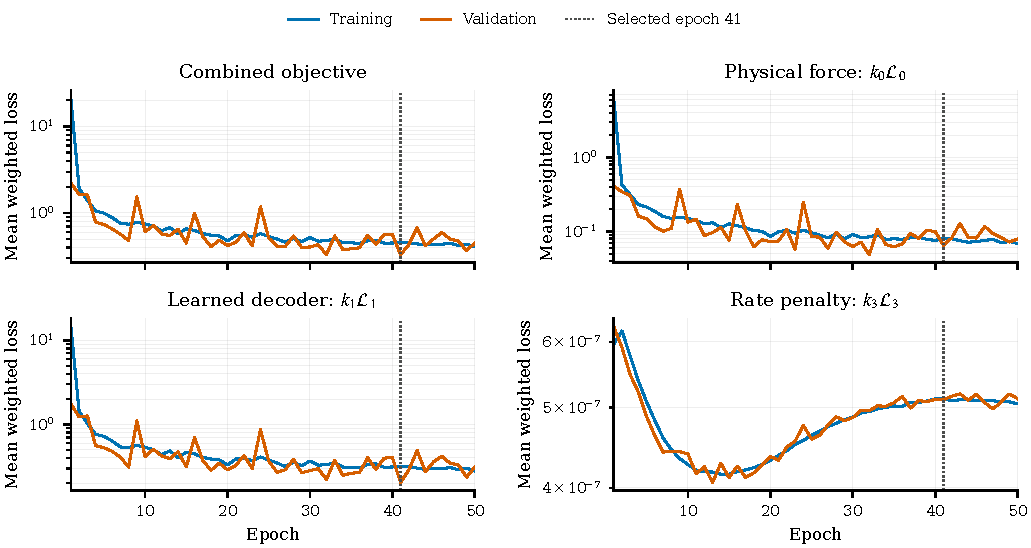
\includegraphics[width=.98\textwidth]{learning_curves}
\caption{Training and validation losses. The dotted line marks the selected
checkpoint. The total includes all six terms; the other panels show
individual weighted terms. Evaluation data are excluded from these curves.}
\label{fig:learning}
\end{figure*}
\begin{figure*}[t]
\centering
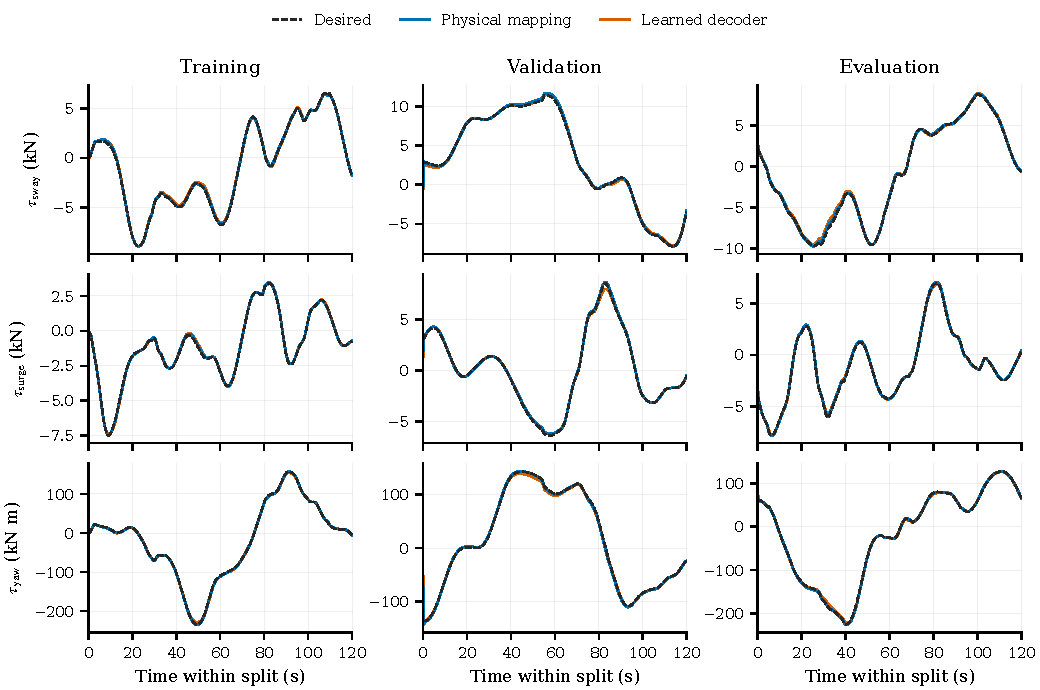
\includegraphics[width=.98\textwidth]{split_reconstruction}
\caption{Force reconstruction over the first 120~s of each split, starting
from zero recurrent memory. Table~\ref{tab:reconstruction} reports errors
for the complete splits.}
\label{fig:reconstruction}
\end{figure*}
\begin{table*}[t]
\caption{Force reconstruction RMSE over each complete data split.}
\label{tab:reconstruction}
\centering
\begin{tabular}{lrrrrrr}
\toprule
&\multicolumn{3}{c}{Physical mapping $\bm g(\uh)$}&\multicolumn{3}{c}{Learned decoder $\tauh$}\\
\cmidrule(lr){2-4}\cmidrule(lr){5-7}
Subset&Sway (N)&Surge (N)&Yaw (N\,m)&Sway (N)&Surge (N)&Yaw (N\,m)\\
\midrule
\inputtable generated/reconstruction_rows.tex
\bottomrule
\end{tabular}
\end{table*}

\section{Experimental Results}
\subsection{Million-sample dataset}
Figure~\ref{fig:commandsdata} shows the generated commands, and
Table~\ref{tab:datarates} reports their peak rates. All samples satisfy
the prescribed sampling magnitude and rate limits.

\begin{table}[t]
\caption{Measured generation rates over all $10^6$ samples.}
\label{tab:datarates}
\centering
\begin{tabular}{lrr}
\toprule
Channel&Peak absolute rate&Allowed rate\\
\midrule
\inputtable generated/data_rate_rows.tex
\bottomrule
\end{tabular}
\end{table}

\subsection{Learning and force reconstruction}
Figure~\ref{fig:learning} shows the mean total loss and three weighted
components over the training epochs. Table~\ref{tab:reconstruction}
reports errors calculated using every sample in each split:
\begin{equation}
 \mathrm{RMSE}_j=\sqrt{\frac{1}{N_s}\sum_{k=1}^{N_s}
       \left(\tau^{\rm out}_{k,j}-\tau^d_{k,j}\right)^2}.
 \label{eq:rmse}
\end{equation}
Here, $\bm\tau^{\rm out}$ is either $\tauc$ or $\tauh$, and $N_s$ is the
number of samples in the split. The physical reconstruction determines
the force applied to the ship; the decoder provides an auxiliary learned
reconstruction. Figure~\ref{fig:reconstruction} compares both outputs
with the desired forces over contiguous portions of all three splits.

Over the complete evaluation subset, the physical reconstruction RMSE
is 86.09~N in sway, 64.66~N in surge, and 1452.47~N\,m in yaw.
Relative to the training standard deviations, these correspond to
1.36\%, 2.31\%, and 1.61\%, respectively. Training and validation errors
are of comparable magnitude. These results apply to the synthetic
trajectory distribution considered here; performance under disturbances
or different operating conditions remains to be evaluated.


Constraint counts for the raw commands are provided in
Table~\ref{tab:offlineconstraints}. Magnitudes are checked against the
physical asymmetric bounds. Rate counts compare adjacent predictions
within each split and exclude the transition from an unspecified initial
actuator setting. Checks use tolerances of $10^{-3}$~N and $10^{-8}$~rad
for command bounds and increments, and $10^{-8}$~rad at sector boundaries.

The evaluation record contains 4,502 actuator--sample rate violations,
although no magnitude or sector violations are observed. Of these rate
violations, 4,150 involve the stern thrusts. The weighted rate loss remains
several orders of magnitude below the force-reconstruction terms,
suggesting that it has limited influence on the training objective.

\begin{table}[t]
\caption{Raw encoder violations over each complete split. Bounds and rates
count actuator--sample violations; sectors count samples with any forbidden
angle. No clipping is applied.}
\label{tab:offlineconstraints}
\centering
\begin{tabular}{lrrr}
\toprule
Subset&Bounds&Rates&Sectors\\
\midrule
\inputtable generated/constraint_rows.tex
\bottomrule
\end{tabular}
\end{table}

\subsection{Allocation time}
On the first 1,024 evaluation requests, the median allocation times are
\NNMedian~ms for the raw neural allocator and \NLPMedian~ms for the NLP.
Measurements use a \CPUModel\ CPU with one PyTorch thread, after ten
warmup calls per method. Timings cover complete allocation calls, including
CasADi problem construction and solver execution for the NLP. They exclude
data loading and ship integration, so the comparison concerns the current
implementations.

\balance
\section{Conclusions}
This work implements a common ship model and thruster mapping for NLP and
recurrent neural control allocation. One million smooth command samples
are generated within prescribed magnitude and rate bounds and divided
chronologically into training, validation, and evaluation subsets. The
encoder outputs three thrust forces and two azimuth angles, while physical
and learned force reconstructions contribute to the training objective.

The neural allocator achieves low force-reconstruction errors and shorter
allocation times than the implemented NLP. However, rate violations remain
despite the soft actuator penalties. Future work should incorporate the
previous applied command and feasible command bounds into training, then
evaluate the allocator on independent trajectories and in closed-loop
positioning tasks.

\bibliographystyle{IEEEtran}
\bibliography{references}
\end{document}
